\section{Wall}
Implementering af Wall widgetten er relativt simpel og indeholder udelukkende enkle CRUD operationer. Wall designes og implementeres som en af de første widgets, idet den er simpel, og dermed giver god indledende erfaring med ASP.NET Core MVC, samt EF Core.

\subsection{2.-4. Iteration}
I 2. iteration oprettes entititerne svarende til dem beskrevet i arkitekturen. Efterfølgende oprettes CRUD views for både Wall og WallPost, som gør det muligt at kunne oprette/redigere/slette Walls og WallPosts. Der lægges vægt på at implementere logikken i controllers så simpelt som muligt, hvilket vil gøre denne nemmere at udvide senere. Efter funktionaliteten virker, tilføjes validering af brugeres adgang, hvilket gøres i iteration 4.

\subsection{6. Iteration}
Når widgets til dashboardet er klar, implementeres det tilhørende view. Heri vises kun de seneste 3 opdaterede posts. Dette gøres for at holde widgetten overskuelig, og ikke fylde for meget. Når pop-up vinduer for at oprette/slette/redigere andre entitieter implementeres, laves disse også for Wall og WallPost. Da alle disse funktionaliteter er tilgængelige både fra Focused og widget-viewet, implementeres det sådan at der omdirigeres til den side hvor funktionen kaldes fra. Et flowchart der beskriver hvordan dette fungerer, kan ses på figur \ref{fig:Wall_Flow}.   

\begin{figure}[H]
  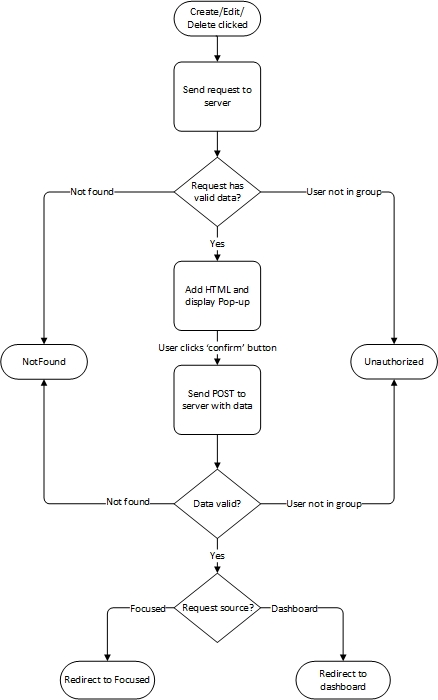
\includegraphics[width=0.8\linewidth]{01_Billeder/10_Design_og_implementering/Wall_Flow.jpg}
  \centering
  \caption{Flowchart der beskriver det overordnede flow i koden for pop-up vinduer til at oprette/slette/redigere WallPosts og Walls}
  \label{fig:Wall_Flow}
\end{figure}


